\documentclass{article}
\usepackage{pgf-pie}
\usepackage{tikz}
\usepackage{enumitem}
\usepackage[top=1.2in,left = 1.7in,right=1.7in]{geometry}
\begin{document}
	\title{Test Problem1}
	\author{Rashi}
	\date{\today}
	\maketitle
	The usage share of web browsers is the proportion, often expressed as a percent-
	age, of visitors to a group of web sites who use a particular web browser.Following
	pie chart shows the percentage of the users who use different web browsers. The
	data is colleted form https://netmarketshare.com/

	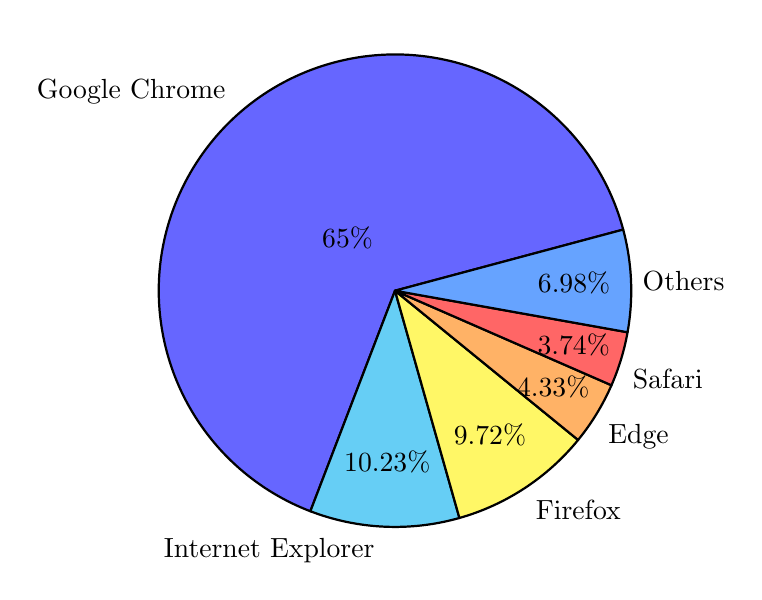
\begin{tikzpicture}
		\pie[rotate=15]{
			65/Google Chrome,10.23/Internet Explorer,9.72/Firefox, 4.33/Edge, 3.74/Safari,6.98/Others
		}
	\end{tikzpicture}\\
	
	\noindent\hrulefill 
	
	\normalsize
	\textbf{Algorithm 1: }Euclid’s algorithm for finding the greatest common di-
	visor of two nonnegative integers
				
	\noindent\hrulefill 
	
	\normalsize 
	%\renewcommand{\baselinestretch}{0.1}
	 \noindent\textbf{1}\hspace{0.25cm}   \underline{function Euclid} $(a,b)$
	  
	\textbf{Input :}Two nonnegative integers a and b
	 
	 \textbf{Output :}gcd$(a,b)$\\
	\textbf{2}\hspace{0.25cm}   \textbf{if }b=0 \textbf{then}\\
	\textbf{3}\hspace{0.25cm}   \textbf{$\mid$} return a\\
	\textbf{4}\hspace{0.25cm}   \textbf{else}\\
	\textbf{5}\hspace{0.25cm}   \textbf{$\mid$}\_ return Euclid($b,a\ mod\ b$)
			
\noindent\hrulefill 

\normalsize
The Euclidean algorithm, also called Euclid’s algorithm, is an algorithm for
finding the greatest common divisor of two numbers a and b. The algorithm\\
\vspace{5cm}

\noindent\hrulefill 

\normalsize
\label{algo}
\textbf{Algorithm 1: }Euclid’s algorithm for finding the greatest common di-
visor of two nonnegative integers

\noindent\hrulefill 

\normalsize 
%\renewcommand{\baselinestretch}{0.1}
\textbf{Input :}$ a, b, c, d$

\textbf{Output :}$e,r$\\
\textbf{1}\hspace{0.25cm}   Calculate $x$ and $y$\\
\textbf{2}\hspace{0.25cm}   \textbf{if} k$\geq$ n  \textbf{then $m_2$}\\
\textbf{3}\\
\textbf{4}\hspace{0.25cm}   \textbf{if} h$\geq$ j  \textbf{then $m_1$}\\
\textbf{5}\\
\textbf{6}\hspace{0.25cm}   \textbf{else}\\ 
\textbf{7}\hspace{0.25cm}   $\mid$ \ \textbf{repeat}\\
\textbf{8}\hspace{0.25cm}   $\mid$ \ $\mid$ \ Initialisation: $g(0) = nj$\\
\textbf{9}\hspace{0.25cm}   $\mid$ \ $\mid$ \ $i = 0$\\
\textbf{10}\hspace{0.05cm}   $\mid$ \ $\mid$ \ Compute $n_2$$$n(i)=\frac{a}{\sqrt{3v}}$$\\
\textbf{11}\hspace{0.05cm}   $\mid$ \ $\mid$ \ Update b $n_2$$$b(i+1)=-\frac{1}{2(g(i))+1}$$\\
\noindent\hrulefill 

\normalsize \noindent
can also be defined for more general rings than just the integers Z. There are
even principal rings which are not Euclidean but where the equivalent of the
Euclidean algorithm can be defined. The algorithm for rational numbers was
given in Book VII of Euclid’s Elements. The algorithm for reals appeared in
Book X, making it the earliest example of an integer relation algorithm.
The \ref{algo} \textbf{Algorithm2} should have to be reffered here.
\end{document}